\chapter{Burndown-Charts}

Die Burndown-Charts zeigen nur vollständigen Issues an.

\section{Sprint 1}

\begin{figure}[H]
	\centering
	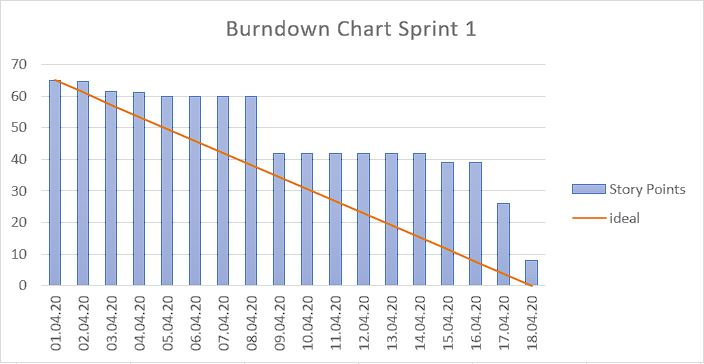
\includegraphics[width=\textwidth]{burndown/sprint1.jpg}
	\caption{Burndowndiagramm Sprint 1}
	\label{figure:burndown_sprint1}
\end{figure}

Im ersten Sprint, vom 01.04.2020 bis zum 18.04.2020, haben wir 65 Storypoints für 20 Issues geschätzt. Am Ende des Sprint ist ein Issue mit 8 Storypoints noch nicht vollständig abgeschlossen gewesen.
\begin{itemize}
\item Scrum Master: Henrik Möhlmann
\item Product Owner: Janik Dohrmann
\end{itemize}

\newpage
\section{Sprint 2}

\begin{figure}[H]
	\centering
	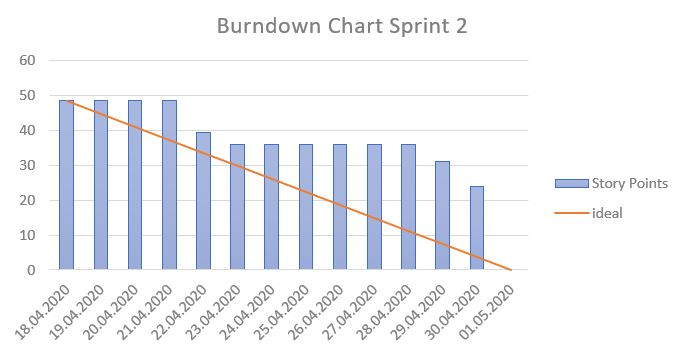
\includegraphics[width=\textwidth]{burndown/sprint2.jpg}
	\caption{Burndowndiagramm Sprint 2}
	\label{figure:burndown_sprint2}
\end{figure}

Im zweiten Sprint, vom 18.04.2020 bis zum 01.05.2020, haben wir 48,5 Storypoints für 11 Issues geschätzt. Am Ende des Sprints waren alle Issues abgearbeitet.
\begin{itemize}
\item Scrum Master: Eric De Ron
\item Product Owner: Florian Müller
\end{itemize}

\newpage
\section{Sprint 3}

\begin{figure}[H]
	\centering
	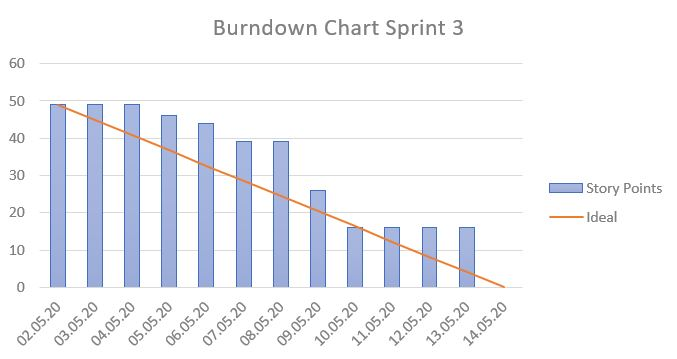
\includegraphics[width=\textwidth]{burndown/sprint3.jpg}
	\caption{Burndowndiagramm Sprint 3}
	\label{figure:burndown_sprint3}
\end{figure}

Im dritten Sprint, vom 02.05.2020 bis zum 14.05.2020, haben wir 49 Storypoints für 10 Issues geschätzt. Am Ende des Sprints waren alle Issues abgearbeitet.
\begin{itemize}
\item Scrum Master: Matthias Hinrichs
\item Product Owner: Alonso Essenwanger
\end{itemize}

\newpage
\section{Sprint 4}

\begin{figure}[H]
	\centering
	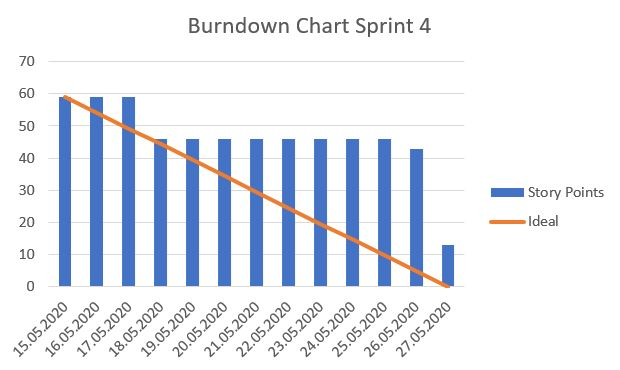
\includegraphics[width=\textwidth]{burndown/sprint4.jpg}
	\caption{Burndowndiagramm Sprint 4}
	\label{figure:burndown_sprint4}
\end{figure}

Im vierten Sprint, vom 15.05.2020 bis zum 27.05.2020, haben wir 59 Storypoints für 9 Issues geschätzt. Am Ende des Sprints ist ein Issue mit 13 Storypoints noch nicht vollständig übergeblieben.
\begin{itemize}
\item Scrum Master: Janik Dohrmann
\item Product Owner: Eric De Ron
\end{itemize}

\newpage
\section{Sprint 5}

\begin{figure}[H]
	\centering
	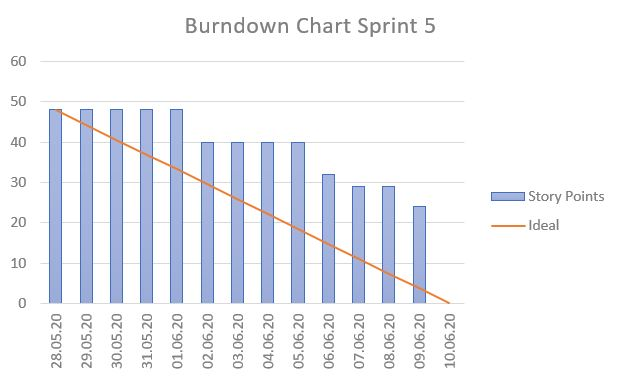
\includegraphics[width=\textwidth]{burndown/sprint5.jpg}
	\caption{Burndowndiagramm Sprint 5}
	\label{figure:burndown_sprint5}
\end{figure}

Im fünften Sprint, vom 28.05.2020 bis zum 10.06.2020, haben wir 48 Storypoints für 7 Issues geschätzt. Am Ende des Sprints waren alle Issues abgearbeitet.
\begin{itemize}
\item Scrum Master: Florian Müller
\item Product Owner: Henrik Möhlmann
\end{itemize}
